
\documentclass[11pt,a4paper,UTF8]{book}

\usepackage[T1]{fontenc}
\usepackage[utf8]{inputenc}
\usepackage{authblk}

\usepackage{fontspec}                  %引入字体设置宏包
\setmainfont{Times New Roman}             %设置英文正文字体
% Courier New
% Book Antique
\setsansfont{Arial}                    %英文无衬线字体
\setmonofont{Courier New}              %英文等宽字体

\usepackage{ctex} %导入中文包
%\usepackage{ulem}
\usepackage{tocvsec2}
\usepackage{verbatim}

\usepackage{tabularx}
\usepackage{booktabs} 
\usepackage{multirow}
\usepackage{bbding}
\usepackage{float}
\usepackage{xspace}
\usepackage[none]{hyphenat}

\usepackage{graphicx}
\usepackage{subfigure}
\usepackage{pifont}

\usepackage{hyperref}  %制作pdf的目录
\usepackage{subfiles} %使用多文件方式进行

\usepackage{geometry} %设置页边距的包
\geometry{left=2.5cm,right=2cm,top=2.54cm,bottom=2.54cm} %设置书籍的页边距

\usepackage{url}
\hypersetup{hidelinks, %去红框
	colorlinks=true,
	allcolors=black,
	pdfstartview=Fit,
	breaklinks=true
}

% 调整itemlist中的行间距
\usepackage{enumitem}
\setenumerate[1]{itemsep=0pt,partopsep=0pt,parsep=\parskip,topsep=5pt}
\setitemize[1]{itemsep=0pt,partopsep=0pt,parsep=\parskip,topsep=5pt}
\setdescription{itemsep=0pt,partopsep=0pt,parsep=\parskip,topsep=5pt}

% 超链接样式设置
\usepackage{hyperref}
\hypersetup{
	colorlinks=true,
	linkcolor=blue,
	filecolor=blue,
	urlcolor=blue,
	citecolor=cyan,
}

\usepackage{indentfirst}

\usepackage{listings}
\usepackage[usenames,dvipsnames,svgnames, x11names]{xcolor}

\usepackage[most]{tcolorbox}
\tcbuselibrary{breakable} % 引入 breakable 库
\tcbuselibrary{skins} % 引入 skins 库

%展示代码
\definecolor{mygreen}{rgb}{0,0.6,0}
\definecolor{mygray}{rgb}{0.5,0.5,0.5}
\definecolor{mymauve}{rgb}{0.58,0,0.82}
\definecolor{keywordcolor}{rgb}{0.8,0.1,0.5}
\definecolor{webgreen}{rgb}{0,.5,0}
\definecolor{bgcolor}{rgb}{0.92,0.92,0.92}

%定义CMake
\lstdefinelanguage{CMake}
{morekeywords={
		cmake\_minimum\_required,
		project,
		add\_executable,
		add\_library,
		target\_link\_libraries,
		cmake\_parse\_arguments,
		cmake\_language,
		set, unset,
		option,
		string,
		list,
		math,
		message,
		if, elseif, else, endif,
		mark\_as\_advanced,
		foreach, endforeach,
		while, endwhile,
		add\_subdirectory, include, return, include\_gurad,
		function, endfunction,
		macro, endmacro,
		find\_package,
		cmake\_push\_check\_state,
		cmake\_pop\_check\_state,
		cmake\_reset\_check\_state,
		add\_test,
		set\_tests\_properties, 
		check\_c\_source\_runs,
		check\_cxx\_source\_runs,
		check\_fortran\_source\_runs,
		check\_source\_runs,
		check\_compiler\_flag,
		check\_c\_compiler\_flag,
		check\_cxx\_compiler\_flag,
		check\_fortran\_compiler\_flag,
		check\_symbol\_exists,
		check\_cxx\_symbol\_exists,
		check\_linker\_flag,
		cmake\_policy,
		set\_property,
		get\_property,
		define\_property,
		get\_cmake\_property,
		set\_cmake\_property,
		set\_target\_properties,
		get\_target\_property,
		set\_directory\_properties,
		get\_directory\_property,
		set\_source\_files\_properties,
		get\_source\_file\_property,
		set\_tests\_properties,
		get\_tests\_property,
		get\_test\_property,
		cmake\_print\_properties,
		cmake\_print\_variables,
		variable\_watch,
		include\_guard,
		target\_link\_options,
		target\_compile\_definitions,
		target\_compile\_options,
		include\_directories,
		add\_definitions,
		remove\_definitions,
		add\_compile\_definitions,
		add\_compile\_options,
		link\_libraries,
		link\_directories,
		add\_link\_options,
		target\_include\_directories,
		target\_compile\_features,
		add\_custom\_command,
		add\_custom\_target,
		execute\_process,
		cmake\_path,
		get\_filename\_component,
		file,
		configure\_file,
		generate\_export\_header,
		export,
		find\_file,
		find\_library,
		find\_package,
		find\_program,
		pkg\_check\_modules,
		pkg\_search\_module,
		pkg\_get\_variable,
		add\_test,
		enable\_testing,
		set\_tests\_properties,
		site\_name,
		ctest\_empty\_binary\_directory,
		ctest\_start,
		ctest\_configure,
		ctest\_submit,
		ctest\_build,
		ctest\_memcheck,
		ctest\_upload,
		ctest\_test,
		gtest\_add\_tests,
		gtest\_discover\_tests,
		install,
		write\_basic\_package\_version\_file,
		configure\_package\_config\_file,
		cpack\_add\_component,
		cpack\_add\_install\_type,
		cpack\_add\_component\_group,
		ExternalProject\_Add,
		ExternalProject\_Add\_StepDependencies,
		ExternalProject\_Get\_Property,
		ExternalProject\_Add\_Step,
		FetchContent\_Declare,
		FetchContent\_GetProperties,
		FetchContent\_Populate,
		source\_group,
		target\_precompile\_headers,
		qt5\_wrap\_cpp,
		qt5\_wrap\_ui,
		qt5\_add\_resources,
		qt5\_add\_big\_resources,
		qt5\_add\_binary\_resources,
		qt5\_add\_translation,
		qt5\_create\_translation,
		compile\_definitions,
		add\_llvm\_component\_library,
		add\_llvm\_tool,
		llvm\_multisource,
		llvm\_test\_data,
		doxygen\_add\_docs,
		cmake\_dependent\_option,
		target\_sources,
		conan\_cmake\_autodetect,
		conan\_cmake\_configure,
		conan\_cmake\_install,
		doxygen\_add\_docs,
		check\_source\_compiles,
		check\_language,
		enable\_language,
		add\_dependencies,
		find\_path,
		find\_package\_handle\_standard\_args,
	}, %定义关键字
	sensitive=false, %是否大小写敏感
	morecomment=[l]{\#},
	morestring=[b]",
	morestring=[d]',
}

\lstdefinestyle{styleCXX}{
	language = C++,  
	backgroundcolor=\color{blue!3!white}, 
	%basicstyle = \footnotesize,  
	basicstyle      =   \zihao{-5}\ttfamily,
	numberstyle     =   \zihao{-5}\ttfamily,   
	%breakatwhitespace = false,    
	basewidth       =   0.5em,    
	breaklines = true,                 
	captionpos = b,                    
	commentstyle = \color{mygray}\bfseries,
	%extendedchars = false,             
	frame =shadowbox, 
	framerule=0.5pt,
	%frameround = fttt,
	keepspaces=true,
	keywordstyle=\color{blue}\bfseries, % keyword style
	otherkeywords={string}, 
	numbers=left, 
	numbersep=5pt,
	numberstyle=\tiny\color{mygray},
	rulecolor=\color{black},         
	%showspaces=false,  
	%showstringspaces=false, 
	%showtabs=false,    
	%stepnumber=1,         
	stringstyle=\color{mymauve},        % string literal style
	tabsize=2,          
	columns         =   fixed,
	flexiblecolumns,                   
}


\lstdefinestyle{styleCMake}{
	language=CMake,
	backgroundcolor=\color{blue!3!white}, 
	basicstyle=\tt, 
	breakatwhitespace = false,
	breaklines = true,
	captionpos = b,
	commentstyle = \color{mygray}\bfseries, 
	extendedchars =false,             
	frame=shadowbox, 
	tabsize=2,
	framerule=0.5pt,
	keepspaces=true,
	keywordstyle=\color{blue}\bfseries, % keyword style
	otherkeywords={string}, 
	rulecolor=\color{black},
	showspaces=false,
	showstringspaces=false,
	showtabs=false,
	stepnumber=1,
	stringstyle=\color{purple},        % string literal style
}

\lstdefinestyle{stylePython}{
	language        =   Python, % 语言选Python
	backgroundcolor=\color{blue!3!white}, 
	basicstyle      =   \zihao{-5}\ttfamily,
	numberstyle     =   \zihao{-5}\ttfamily,
	keywordstyle    =   \color{blue},
	keywordstyle    =   [2] \color{teal},
	stringstyle     =   \color{magenta},
	commentstyle    =   \color{red}\ttfamily,
	frame = shadowbox, 
	breaklines      =   true,   % 自动换行,建议不要写太长的行
	columns         =   fixed,  % 如果不加这一句,字间距就不固定,很丑,必须加
	basewidth       =   0.5em,
	%basicstyle          =   \sffamily,          % 基本代码风格
	%keywordstyle        =   \bfseries,          % 关键字风格
	%commentstyle        =   \rmfamily\itshape,  % 注释的风格,斜体
	%stringstyle         =   \ttfamily,  % 字符串风格
	flexiblecolumns,                % 别问为什么,加上这个
	%numbers             =   left,   % 行号的位置在左边
	showspaces          =   false,  % 是否显示空格,显示了有点乱,所以不现实了
	numberstyle         =   \zihao{-5}\ttfamily,    % 行号的样式,小五号,tt等宽字体
	showstringspaces    =   false,
	captionpos          =   t,      % 这段代码的名字所呈现的位置,t指的是top上面
	frame               =   lrtb,   % 显示边框
	tabsize=2,  
}

\tcbset{
	breakable,
	commandshell/.style={
		listing only,
		colback=black!75!white,
		colupper=white,
		lowerbox=ignored,
		listing options={
			language={bash},
			breaklines=true,
			basicstyle=\ttfamily,
			columns = fixed,
			flexiblecolumns
		}
}}

\usepackage{tikz}

% URL 正确换行
% https://liam.page/2017/05/17/help-the-url-command-from-hyperref-to-break-at-line-wrapping-point/
\makeatletter
\def\UrlAlphabet{%
	\do\a\do\b\do\c\do\d\do\e\do\f\do\g\do\h\do\i\do\j%
	\do\k\do\l\do\m\do\n\do\o\do\p\do\q\do\r\do\s\do\t%
	\do\u\do\v\do\w\do\x\do\y\do\z\do\A\do\B\do\C\do\D%
	\do\E\do\F\do\G\do\H\do\I\do\J\do\K\do\L\do\M\do\N%
	\do\O\do\P\do\Q\do\R\do\S\do\T\do\U\do\V\do\W\do\X%
	\do\Y\do\Z}
\def\UrlDigits{\do\1\do\2\do\3\do\4\do\5\do\6\do\7\do\8\do\9\do\0}
\g@addto@macro{\UrlBreaks}{\UrlOrds}
\g@addto@macro{\UrlBreaks}{\UrlAlphabet}
\g@addto@macro{\UrlBreaks}{\UrlDigits}
\makeatother

% enable subsubsubsection
% from https://tex.stackexchange.com/练习题/274212/correct-hierarchy-levels-of-pdf-bookmarks-for-custom-section-subsubsubsection
\usepackage[depth=3]{bookmark}
\setcounter{secnumdepth}{3}
\setcounter{tocdepth}{4}
\hypersetup{bookmarksdepth=4}

\makeatletter

\newcommand{\toclevel@subsubsubsection}{4}
\newcounter{subsubsubsection}[subsubsection]

\renewcommand{\thesubsubsubsection}{\thesubsubsection.\arabic{subsubsubsection}}

\newcommand{\subsubsubsection}{\@startsection{subsubsubsection}{4}{\z@}%
	{-3.25ex\@plus -1ex \@minus -.2ex}%
	{1.5ex \@plus .2ex}%
	{\normalfont\normalsize\bf\bfseries}}

\newcommand*{\l@subsubsubsection}{\@dottedtocline{4}{11em}{5em}}  

\newcommand{\subsubsubsectionmark}[1]{}
\makeatother

\begin{document}
	\begin{sloppypar} %latex中一行文字出现溢出问题的解决方法
		%\maketitle
		
		\begin{center}
			\thispagestyle{empty}
			%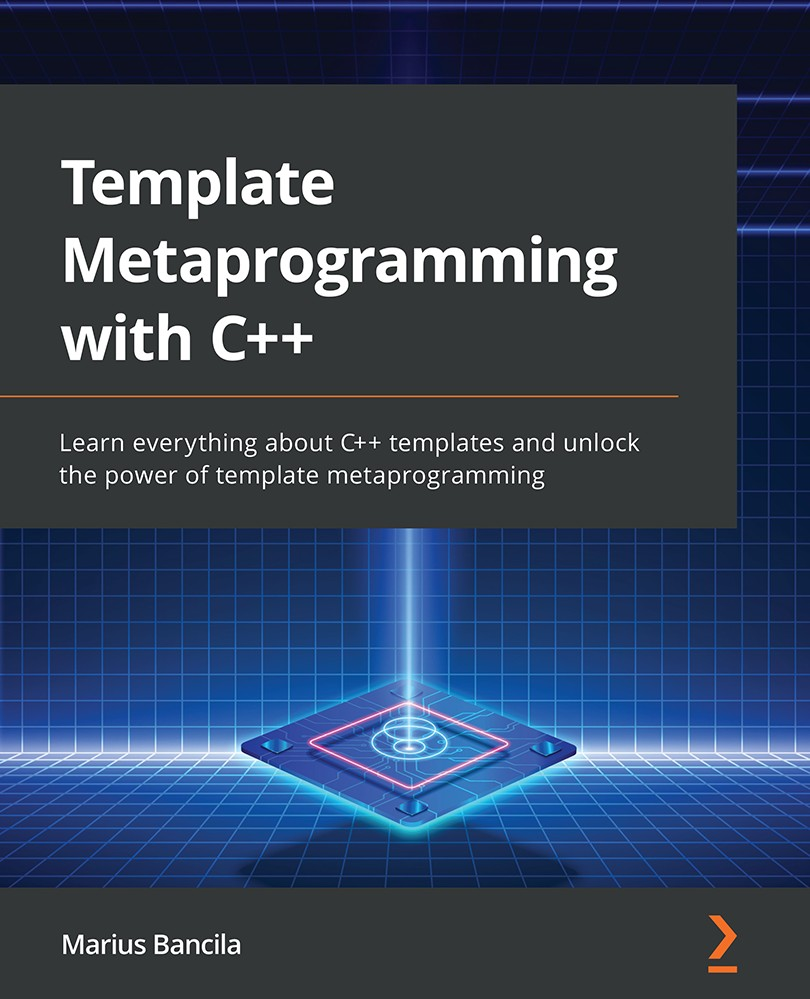
\includegraphics[width=\textwidth,height=\textheight,keepaspectratio]{cover.jpg}
			\begin{tikzpicture}[remember picture, overlay, inner sep=0pt]
				\node at (current page.center) 
				{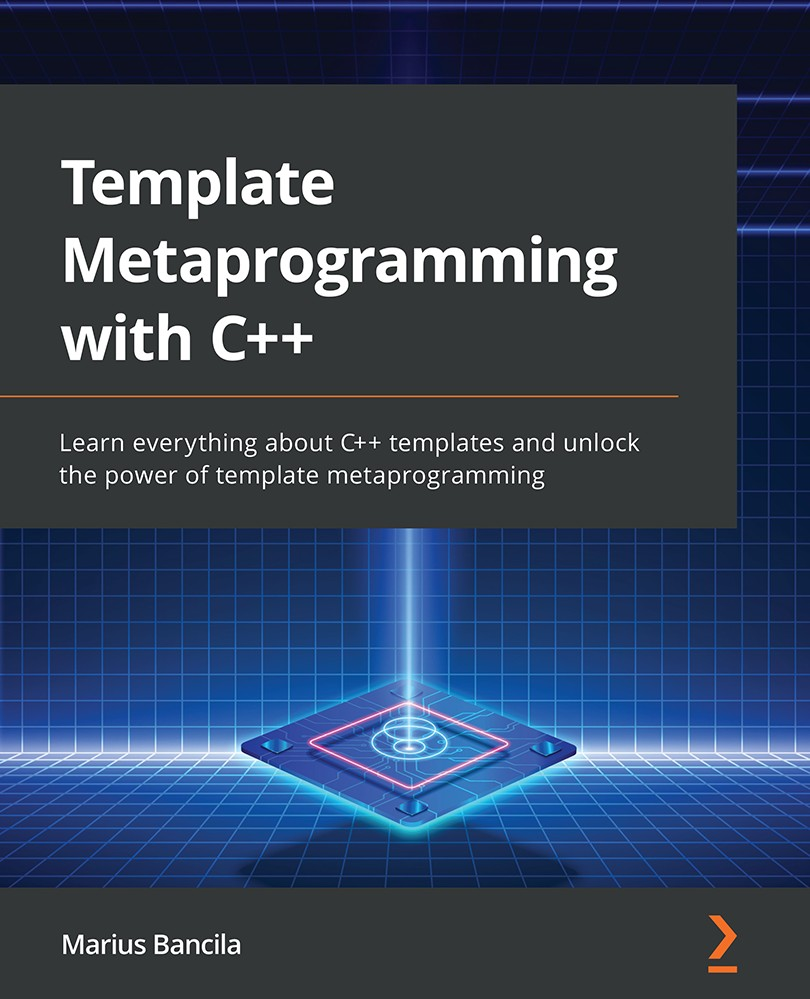
\includegraphics[width=\paperwidth, keepaspectratio=false]{cover.jpg}};
			\end{tikzpicture}
			\newpage
			\thispagestyle{empty}
			\huge
			\textbf{Template Metaprogramming with C++} 
			\\[9pt]
			\normalsize
			\textit{Learn everything about C++ templates and unlock the power of template metaprogramming \\ 详细的了解C++模板,解锁模板元编程的力量}
			\\[10pt]
			\normalsize 
			作者: Marius Bancila 
			\\[8pt]
			\normalsize
			译者:陈晓伟
		\end{center}
		
		\hspace*{\fill} \\ %插入空行
		\noindent\textbf{本书概述}
		
		了解元编程技术,从而能够创建在编译时进行计算的数据结构和函数。通过这本书,您将了解模板如何避免编写重复的代码,并且作为创建通用库(如标准库或Boost)的关键(这些通用库可用于许多程序中)。
		
		本书将带您深入了解模板和元编程的基础知识,再练习编写复杂的模板,并探索高级概念,如模板递归、模板参数推导、转发引用、类型特征和条件编译。在此过程中,将了解如何编写可变参数模板,以及如何使用C++20约束和概念为模板参数进行限制。最后,可以使用C++元编程模板的知识来实现各种元编程模式和技术。
		
		本书的最后,将学习如何在日常编程之旅中编写有效的模板和实现元编程。
		
		\hspace*{\fill} \\ %插入空行
		\noindent\textbf{关键特性}
		\begin{itemize}
			\item 了解C++20的最新特性,并使用STL编写更好的代码
			\item 减少应用程序的开发时间,并更快的进行部署
			\item 使用最新标准中引入的新的、精简的STL功能
		\end{itemize}
		
		\hspace*{\fill} \\ %插入空行
		\noindent\textbf{将会学到}
		\begin{itemize}
			\item 了解所有类型模板的语法
			\item 了解特化和实例化如何工作
			\item 掌握模板参数推断和转发引用
			\item 轻松编写可变模板
			\item 熟悉类型特征和条件编译
			\item 用约束和概念限制C++20中的模板参数
			\item 实现CRTP、mixins和标签调度等模式
		\end{itemize}
	
		\hspace*{\fill} \\ %插入空行
		\noindent\textbf{适读人群}
		这本书是为初学者到中级C++开发人员(学习模板元编程),以及高级C++开发人员,希望了解与模板相关的新C++ 20特性、习语和模式。开始阅读这本书前,需要对基本的C++编程有所了解。
		
		\hspace*{\fill} \\ %插入空行
		\noindent\textbf{作者简介}
		
		\textbf{Marius Bancila}是一名软件工程师,为工业和金融部门开发解决方案方面,拥有近20年的经验。他是《现代C++挑战》的作者和《学习C\#编程》的合著者。并且是一名软件架构师,专注于Microsoft技术,主要使用C++和C\#开发桌面应用程序。他热衷于与他人分享他的技术专长,自2006年以来,他一直是微软C++和开发人员眼中的技术MVP。Marius住在罗马尼亚,并且活跃在各种网络社区。
		
		\hspace*{\fill} \\ %插入空行
		\noindent\textbf{审阅者简介}
	
		\textbf{Aleksei Goriachikh}使用的C++编程超过8年。Aleksei于2012年从新西伯利亚州立大学(Novosibirsk State University)数学硕士学位毕业后,之后一直从事计算数学和优化、CAD系统的几何核,以及自动驾驶的多线程实现等领域的研究。Aleksei目前的兴趣是前硅建模。
		
		\hspace*{\fill} \\ %插入空行
		\noindent\textbf{本书相关}
		\begin{itemize}
			\item Github地址:
			\url{https://github.com/xiaoweiChen/Template-Metaprogramming-with-CPP}
		\end{itemize}
		\newpage
		
		\vspace*{\fill}
		\begin{center}
		\textit{献给自己那“该死的”好奇心。}
		
		\textit{– Marius Bancila}
		\end{center}
		\vspace*{\fill}
		\newpage
		
		%前言
		\pagestyle{empty}
		\subfile{content/preface.tex}
		\newpage
		
		\tableofcontents
		\newpage
		
		\setsecnumdepth{section}
		
		\color{white}
		\section*{\zihao{1}第一部分:模板的核心概念}
		\pagecolor{mygray}
		\addcontentsline{toc}{section}{第一部分:模板的核心概念}
		\textbf{\subfile{content/1/section.tex}}
		\newpage
		\color{black}
		\pagecolor{white}
		
		\subsection*{\zihao{2} 第1章\hspace{0.5cm}模板简介}
		\addcontentsline{toc}{subsection}{第1章\hspace{0.5cm}模板简介}
		\subfile{content/1/chapter1/0.tex}
		
		\subsubsection*{\zihao{3} 1.1.\hspace{0.2cm}使用模板的动机}
		\addcontentsline{toc}{subsubsection}{1.1.\hspace{0.2cm}使用模板的动机}
		\subfile{content/1/chapter1/1.tex}
		
		\subsubsection*{\zihao{3} 1.2.\hspace{0.2cm}编写模板}
		\addcontentsline{toc}{subsubsection}{1.2.\hspace{0.2cm}编写模板}
		\subfile{content/1/chapter1/2.tex}
		
		\subsubsection*{\zihao{3} 1.3.\hspace{0.2cm}理解模板}
		\addcontentsline{toc}{subsubsection}{1.3.\hspace{0.2cm}理解模板}
		\subfile{content/1/chapter1/3.tex}
		
		\subsubsection*{\zihao{3} 1.4.\hspace{0.2cm}模板简史}
		\addcontentsline{toc}{subsubsection}{1.4.\hspace{0.2cm}模板简史}
		\subfile{content/1/chapter1/4.tex}
		
		\subsubsection*{\zihao{3} 1.5.\hspace{0.2cm}模板的优缺点}
		\addcontentsline{toc}{subsubsection}{1.5.\hspace{0.2cm}模板的优缺点}
		\subfile{content/1/chapter1/5.tex}
		
		\subsubsection*{\zihao{3} 1.6.\hspace{0.2cm}总结}
		\addcontentsline{toc}{subsubsection}{1.6.\hspace{0.2cm}总结}
		\subfile{content/1/chapter1/6.tex}
		
		\subsubsection*{\zihao{3} 1.7.\hspace{0.2cm}习题}
		\addcontentsline{toc}{subsubsection}{1.7.\hspace{0.2cm}习题}
		\subfile{content/1/chapter1/7.tex}
		
		\subsubsection*{\zihao{3} 1.8.\hspace{0.2cm}扩展阅读}
		\addcontentsline{toc}{subsubsection}{1.8.\hspace{0.2cm}扩展阅读}
		\subfile{content/1/chapter1/8.tex}
		\newpage
		
		\subsection*{\zihao{2} 第2章\hspace{0.5cm}了解模板}
		\addcontentsline{toc}{subsection}{第2章\hspace{0.5cm}了解模板}
		\subfile{content/1/chapter2/0.tex}
		
		\subsubsection*{\zihao{3} 2.1.\hspace{0.2cm}定义函数模板}
		\addcontentsline{toc}{subsubsection}{2.1.\hspace{0.2cm}定义函数模板}
		\subfile{content/1/chapter2/1.tex}
		
		\subsubsection*{\zihao{3} 2.2.\hspace{0.2cm}定义类模板}
		\addcontentsline{toc}{subsubsection}{2.2.\hspace{0.2cm}定义类模板}
		\subfile{content/1/chapter2/2.tex}
		
		\subsubsection*{\zihao{3} 2.3.\hspace{0.2cm}定义成员函数模板}
		\addcontentsline{toc}{subsubsection}{2.3.\hspace{0.2cm}定义成员函数模板}
		\subfile{content/1/chapter2/3.tex}
		
		\subsubsection*{\zihao{3} 2.4.\hspace{0.2cm}模板参数}
		\addcontentsline{toc}{subsubsection}{2.4.\hspace{0.2cm}模板参数}
		\subfile{content/1/chapter2/4.tex}
		
		\subsubsection*{\zihao{3} 2.5.\hspace{0.2cm}模板实例化}
		\addcontentsline{toc}{subsubsection}{2.5.\hspace{0.2cm}模板实例化}
		\subfile{content/1/chapter2/5.tex}
		
		\subsubsection*{\zihao{3} 2.6.\hspace{0.2cm}模板特化}
		\addcontentsline{toc}{subsubsection}{2.6.\hspace{0.2cm}模板特化}
		\subfile{content/1/chapter2/6.tex}
		
		\subsubsection*{\zihao{3} 2.7.\hspace{0.2cm}定义变量模板}
		\addcontentsline{toc}{subsubsection}{2.7.\hspace{0.2cm}定义变量模板}
		\subfile{content/1/chapter2/7.tex}
		
		\subsubsection*{\zihao{3} 2.8.\hspace{0.2cm}定义别名模板}
		\addcontentsline{toc}{subsubsection}{2.8.\hspace{0.2cm}定义别名模板}
		\subfile{content/1/chapter2/8.tex}
		
		\subsubsection*{\zihao{3} 2.9.\hspace{0.2cm}通用Lambda和Lambda模板}
		\addcontentsline{toc}{subsubsection}{2.9.\hspace{0.2cm}通用Lambda和Lambda模板}
		\subfile{content/1/chapter2/9.tex}
		
		\subsubsection*{\zihao{3} 2.10.\hspace{0.2cm}总结}
		\addcontentsline{toc}{subsubsection}{2.10.\hspace{0.2cm}总结}
		\subfile{content/1/chapter2/10.tex}
		
		\subsubsection*{\zihao{3} 2.11.\hspace{0.2cm}习题}
		\addcontentsline{toc}{subsubsection}{2.11.\hspace{0.2cm}习题}
		\subfile{content/1/chapter2/11.tex}
		
		\subsubsection*{\zihao{3} 2.12.\hspace{0.2cm}扩展阅读}
		\addcontentsline{toc}{subsubsection}{2.12.\hspace{0.2cm}扩展阅读}
		\subfile{content/1/chapter2/12.tex}
		\newpage
		
		\subsection*{\zihao{2} 第3章\hspace{0.5cm}可变参数模板}
		\addcontentsline{toc}{subsection}{第3章\hspace{0.5cm}可变参数模板}
		\subfile{content/1/chapter3/0.tex}
		
		\subsubsection*{\zihao{3} 3.1.\hspace{0.2cm}可变参数模板的需求}
		\addcontentsline{toc}{subsubsection}{3.1.\hspace{0.2cm}可变参数模板的需求}
		\subfile{content/1/chapter3/1.tex}
		
		\subsubsection*{\zihao{3} 3.2.\hspace{0.2cm}可变参数函数模板}
		\addcontentsline{toc}{subsubsection}{3.2.\hspace{0.2cm}可变参数函数模板}
		\subfile{content/1/chapter3/2.tex}
		
		\subsubsection*{\zihao{3} 3.3.\hspace{0.2cm}参数包}
		\addcontentsline{toc}{subsubsection}{3.3.\hspace{0.2cm}参数包}
		\subfile{content/1/chapter3/3.tex}
		
		\subsubsection*{\zihao{3} 3.4.\hspace{0.2cm}可变参数类模板}
		\addcontentsline{toc}{subsubsection}{3.4.\hspace{0.2cm}可变参数类模板}
		\subfile{content/1/chapter3/4.tex}
		
		\subsubsection*{\zihao{3} 3.5.\hspace{0.2cm}折叠表达式}
		\addcontentsline{toc}{subsubsection}{3.5.\hspace{0.2cm}折叠表达式}
		\subfile{content/1/chapter3/5.tex}
		
		\subsubsection*{\zihao{3} 3.6.\hspace{0.2cm}可变参数别名模板}
		\addcontentsline{toc}{subsubsection}{3.6.\hspace{0.2cm}可变参数别名模板}
		\subfile{content/1/chapter3/6.tex}
		
		\subsubsection*{\zihao{3} 3.7.\hspace{0.2cm}可变参数变量模板}
		\addcontentsline{toc}{subsubsection}{3.7.\hspace{0.2cm}可变参数变量模板}
		\subfile{content/1/chapter3/7.tex}
		
		\subsubsection*{\zihao{3} 3.8.\hspace{0.2cm}总结}
		\addcontentsline{toc}{subsubsection}{3.8.\hspace{0.2cm}总结}
		\subfile{content/1/chapter3/8.tex}
		
		\subsubsection*{\zihao{3} 3.9.\hspace{0.2cm}习题}
		\addcontentsline{toc}{subsubsection}{3.9.\hspace{0.2cm}习题}
		\subfile{content/1/chapter3/9.tex}
		
		\subsubsection*{\zihao{3} 3.10.\hspace{0.2cm}扩展阅读}
		\addcontentsline{toc}{subsubsection}{3.10.\hspace{0.2cm}扩展阅读}
		\subfile{content/1/chapter3/10.tex}
		\newpage
		
		\color{white}
		\section*{\zihao{1}第二部分:模板进阶特性}
		\pagecolor{mygray}
		\addcontentsline{toc}{section}{第二部分:模板进阶特性}
		\textbf{\subfile{content/2/section.tex}}
		\newpage
		\color{black}
		\pagecolor{white}
		
		\subsection*{\zihao{2} 第4章\hspace{0.5cm}高级模板概念}
		\addcontentsline{toc}{subsection}{第4章\hspace{0.5cm}高级模板概念}
		\subfile{content/2/chapter4/0.tex}
		
		\subsubsection*{\zihao{3} 4.1.\hspace{0.2cm}名称绑定和依赖名称}
		\addcontentsline{toc}{subsubsection}{4.1.\hspace{0.2cm}名称绑定和依赖名称}
		\subfile{content/2/chapter4/1.tex}
		
		\subsubsection*{\zihao{3} 4.2.\hspace{0.2cm}模板递归}
		\addcontentsline{toc}{subsubsection}{4.2.\hspace{0.2cm}模板递归}
		\subfile{content/2/chapter4/2.tex}
		
		\subsubsection*{\zihao{3} 4.3.\hspace{0.2cm}函数模板的参数推导}
		\addcontentsline{toc}{subsubsection}{4.3.\hspace{0.2cm}函数模板的参数推导}
		\subfile{content/2/chapter4/3.tex}
		
		\subsubsection*{\zihao{3} 4.4.\hspace{0.2cm}类模板的参数推导}
		\addcontentsline{toc}{subsubsection}{4.4.\hspace{0.2cm}类模板的参数推导}
		\subfile{content/2/chapter4/4.tex}
		
		\subsubsection*{\zihao{3} 4.5.\hspace{0.2cm}转发引用}
		\addcontentsline{toc}{subsubsection}{4.5.\hspace{0.2cm}转发引用}
		\subfile{content/2/chapter4/5.tex}
		
		\subsubsection*{\zihao{3} 4.6.\hspace{0.2cm}decltype说明符}
		\addcontentsline{toc}{subsubsection}{4.6.\hspace{0.2cm}decltype说明符}
		\subfile{content/2/chapter4/6.tex}
		
		\subsubsection*{\zihao{3} 4.7.\hspace{0.2cm}std::declval类型操作符}
		\addcontentsline{toc}{subsubsection}{4.7.\hspace{0.2cm}std::declval类型操作符}
		\subfile{content/2/chapter4/7.tex}
		
		\subsubsection*{\zihao{3} 4.8.\hspace{0.2cm}模板间的“友情”}
		\addcontentsline{toc}{subsubsection}{4.8.\hspace{0.2cm}模板间的“友情”}
		\subfile{content/2/chapter4/8.tex}
		
		\subsubsection*{\zihao{3} 4.9.\hspace{0.2cm}总结}
		\addcontentsline{toc}{subsubsection}{4.9.\hspace{0.2cm}总结}
		\subfile{content/2/chapter4/9.tex}
		
		\subsubsection*{\zihao{3} 4.10.\hspace{0.2cm}习题}
		\addcontentsline{toc}{subsubsection}{4.10.\hspace{0.2cm}习题}
		\subfile{content/2/chapter4/10.tex}
		
		\subsubsection*{\zihao{3} 4.11.\hspace{0.2cm}扩展阅读}
		\addcontentsline{toc}{subsubsection}{4.11.\hspace{0.2cm}扩展阅读}
		\subfile{content/2/chapter4/11.tex}
		\newpage
		
		\subsection*{\zihao{2} 第5章\hspace{0.5cm}类型特征和条件编译}
		\addcontentsline{toc}{subsection}{第5章\hspace{0.5cm}类型特征和条件编译}
		\subfile{content/2/chapter5/0.tex}
		
		\subsubsection*{\zihao{3} 5.1.\hspace{0.2cm}定义类型特征}
		\addcontentsline{toc}{subsubsection}{5.1.\hspace{0.2cm}定义类型特征}
		\subfile{content/2/chapter5/1.tex}
		
		\subsubsection*{\zihao{3} 5.2.\hspace{0.2cm}了解SFINAE}
		\addcontentsline{toc}{subsubsection}{5.2.\hspace{0.2cm}了解SFINAE}
		\subfile{content/2/chapter5/2.tex}
		
		\subsubsection*{\zihao{3} 5.3.\hspace{0.2cm}使用enable\_if类型特性启用SFINAE}
		\addcontentsline{toc}{subsubsection}{5.3.\hspace{0.2cm}使用enable\_if类型特性启用SFINAE}
		\subfile{content/2/chapter5/3.tex}
		
		\subsubsection*{\zihao{3} 5.4.\hspace{0.2cm}constexpr if}
		\addcontentsline{toc}{subsubsection}{5.4.\hspace{0.2cm}constexpr if}
		\subfile{content/2/chapter5/4.tex}
		
		\subsubsection*{\zihao{3} 5.5.\hspace{0.2cm}探索标准类型特征}
		\addcontentsline{toc}{subsubsection}{5.5.\hspace{0.2cm}探索标准类型特征}
		\subfile{content/2/chapter5/5.tex}
		
		\subsubsection*{\zihao{3} 5.6.\hspace{0.2cm}实际使用类型特征的例子}
		\addcontentsline{toc}{subsubsection}{5.6.\hspace{0.2cm}实际使用类型特征的例子}
		\subfile{content/2/chapter5/6.tex}
		
		\subsubsection*{\zihao{3} 5.7.\hspace{0.2cm}总结}
		\addcontentsline{toc}{subsubsection}{5.7.\hspace{0.2cm}总结}
		\subfile{content/2/chapter5/7.tex}
		
		\subsubsection*{\zihao{3} 5.8.\hspace{0.2cm}习题}
		\addcontentsline{toc}{subsubsection}{5.8.\hspace{0.2cm}习题}
		\subfile{content/2/chapter5/8.tex}
		
		\subsubsection*{\zihao{3} 5.9.\hspace{0.2cm}扩展阅读}
		\addcontentsline{toc}{subsubsection}{5.9.\hspace{0.2cm}扩展阅读}
		\subfile{content/2/chapter5/9.tex}
		\newpage
		
		\subsection*{\zihao{2} 第6章\hspace{0.5cm}概念和约束}
		\addcontentsline{toc}{subsection}{第6章\hspace{0.5cm}概念和约束}
		\subfile{content/2/chapter6/0.tex}
		
		\subsubsection*{\zihao{3} 6.1.\hspace{0.2cm}概念的需求}
		\addcontentsline{toc}{subsubsection}{6.1.\hspace{0.2cm}概念的需求}
		\subfile{content/2/chapter6/1.tex}
		
		\subsubsection*{\zihao{3} 6.2.\hspace{0.2cm}定义概念}
		\addcontentsline{toc}{subsubsection}{6.2.\hspace{0.2cm}定义概念}
		\subfile{content/2/chapter6/2.tex}
		
		\subsubsection*{\zihao{3} 6.3.\hspace{0.2cm}探索require表达式}
		\addcontentsline{toc}{subsubsection}{6.3.\hspace{0.2cm}探索require表达式}
		\subfile{content/2/chapter6/3.tex}
		
		\subsubsection*{\zihao{3} 6.4.\hspace{0.2cm}组合约束}
		\addcontentsline{toc}{subsubsection}{6.4.\hspace{0.2cm}组合约束}
		\subfile{content/2/chapter6/4.tex}
		
		\subsubsection*{\zihao{3} 6.5.\hspace{0.2cm}模板中约束的顺序}
		\addcontentsline{toc}{subsubsection}{6.5.\hspace{0.2cm}模板中约束的顺序}
		\subfile{content/2/chapter6/5.tex}
		
		\subsubsection*{\zihao{3} 6.6.\hspace{0.2cm}约束非模板成员函数}
		\addcontentsline{toc}{subsubsection}{6.6.\hspace{0.2cm}约束非模板成员函数}
		\subfile{content/2/chapter6/6.tex}
		
		\subsubsection*{\zihao{3} 6.7.\hspace{0.2cm}约束类模板}
		\addcontentsline{toc}{subsubsection}{6.7.\hspace{0.2cm}约束类模板}
		\subfile{content/2/chapter6/7.tex}
		
		\subsubsection*{\zihao{3} 6.8.\hspace{0.2cm}约束变量模板和模板别名}
		\addcontentsline{toc}{subsubsection}{6.8.\hspace{0.2cm}约束变量模板和模板别名}
		\subfile{content/2/chapter6/8.tex}
		
		\subsubsection*{\zihao{3} 6.9.\hspace{0.2cm}更多指定约束的方法}
		\addcontentsline{toc}{subsubsection}{6.9.\hspace{0.2cm}更多指定约束的方法}
		\subfile{content/2/chapter6/9.tex}
		
		\subsubsection*{\zihao{3} 6.10.\hspace{0.2cm}使用概念来约束auto参数}
		\addcontentsline{toc}{subsubsection}{6.10.\hspace{0.2cm}使用概念来约束auto参数}
		\subfile{content/2/chapter6/10.tex}
		
		\subsubsection*{\zihao{3} 6.11.\hspace{0.2cm}探索标准概念库}
		\addcontentsline{toc}{subsubsection}{6.11.\hspace{0.2cm}探索标准概念库}
		\subfile{content/2/chapter6/11.tex}
		
		\subsubsection*{\zihao{3} 6.12.\hspace{0.2cm}总结}
		\addcontentsline{toc}{subsubsection}{6.12.\hspace{0.2cm}总结}
		\subfile{content/2/chapter6/12.tex}
		
		\subsubsection*{\zihao{3} 6.13.\hspace{0.2cm}习题}
		\addcontentsline{toc}{subsubsection}{6.13.\hspace{0.2cm}习题}
		\subfile{content/2/chapter6/13.tex}
		
		\subsubsection*{\zihao{3} 6.14.\hspace{0.2cm}扩展阅读}
		\addcontentsline{toc}{subsubsection}{6.14.\hspace{0.2cm}扩展阅读}
		\subfile{content/2/chapter6/14.tex}
		\newpage
		
		\color{white}
		\section*{\zihao{1}第三部分:模板的应用}
		\pagecolor{mygray}
		\addcontentsline{toc}{section}{第三部分:模板的应用}
		\textbf{\subfile{content/3/section.tex}}
		\newpage
		\color{black}
		\pagecolor{white}
		
		\subsection*{\zihao{2} 第7章\hspace{0.5cm}模式和习语}
		\addcontentsline{toc}{subsection}{第7章\hspace{0.5cm}模式和习语}
		\subfile{content/3/chapter7/0.tex}
		
		\subsubsection*{\zihao{3} 7.1.\hspace{0.2cm}Dynamic versus static polymorphism}
		\addcontentsline{toc}{subsubsection}{7.1.\hspace{0.2cm}Dynamic versus static polymorphism}
		\subfile{content/3/chapter7/1.tex}
		
		\subsubsection*{\zihao{3} 7.2.\hspace{0.2cm}The Curiously Recurring Template Pattern}
		\addcontentsline{toc}{subsubsection}{7.2.\hspace{0.2cm}The Curiously Recurring Template Pattern}
		\subfile{content/3/chapter7/2.tex}
		
		\subsubsection*{\zihao{3} 7.3.\hspace{0.2cm}Mixins}
		\addcontentsline{toc}{subsubsection}{7.3.\hspace{0.2cm}Mixins}
		\subfile{content/3/chapter7/3.tex}
		
		\subsubsection*{\zihao{3} 7.4.\hspace{0.2cm}Type erasure}
		\addcontentsline{toc}{subsubsection}{7.4.\hspace{0.2cm}Type erasure}
		\subfile{content/3/chapter7/4.tex}
		
		\subsubsection*{\zihao{3} 7.5.\hspace{0.2cm}Tag dispatching}
		\addcontentsline{toc}{subsubsection}{7.5.\hspace{0.2cm}Tag dispatching}
		\subfile{content/3/chapter7/5.tex}
		
		\subsubsection*{\zihao{3} 7.6.\hspace{0.2cm}Expression templates}
		\addcontentsline{toc}{subsubsection}{7.6.\hspace{0.2cm}Expression templates}
		\subfile{content/3/chapter7/6.tex}
		
		\subsubsection*{\zihao{3} 7.7.\hspace{0.2cm}Typelists}
		\addcontentsline{toc}{subsubsection}{7.7.\hspace{0.2cm}Typelists}
		\subfile{content/3/chapter7/7.tex}
		
		\subsubsection*{\zihao{3} 7.8.\hspace{0.2cm}总结}
		\addcontentsline{toc}{subsubsection}{7.8.\hspace{0.2cm}总结}
		\subfile{content/3/chapter7/8.tex}
		
		\subsubsection*{\zihao{3} 7.9.\hspace{0.2cm}习题}
		\addcontentsline{toc}{subsubsection}{7.9.\hspace{0.2cm}习题}
		\subfile{content/3/chapter7/9.tex}
		
		\subsubsection*{\zihao{3} 7.10.\hspace{0.2cm}扩展阅读}
		\addcontentsline{toc}{subsubsection}{7.10.\hspace{0.2cm}扩展阅读}
		\subfile{content/3/chapter7/10.tex}
		\newpage
		
		\subsection*{\zihao{2} 第8章\hspace{0.5cm}范围和算法}
		\addcontentsline{toc}{subsection}{第8章\hspace{0.5cm}范围和算法}
		\subfile{content/3/chapter8/0.tex}
		
		\subsubsection*{\zihao{3} 8.1.\hspace{0.2cm}Understanding the design of containers, iterators, and algorithms}
		\addcontentsline{toc}{subsubsection}{8.1.\hspace{0.2cm}Understanding the design of containers, iterators, and algorithms}
		\subfile{content/3/chapter8/1.tex}
		
		\subsubsection*{\zihao{3} 8.2.\hspace{0.2cm}Creating a custom container and iterator}
		\addcontentsline{toc}{subsubsection}{8.2.\hspace{0.2cm}Creating a custom container and iterator}
		\subfile{content/3/chapter8/2.tex}
		
		\subsubsection*{\zihao{3} 8.3.\hspace{0.2cm}Writing a custom general-purpose algorithm}
		\addcontentsline{toc}{subsubsection}{8.3.\hspace{0.2cm}Writing a custom general-purpose algorithm}
		\subfile{content/3/chapter8/3.tex}
		
		\subsubsection*{\zihao{3} 8.4.\hspace{0.2cm}总结}
		\addcontentsline{toc}{subsubsection}{8.4.\hspace{0.2cm}总结}
		\subfile{content/3/chapter8/4.tex}
		
		\subsubsection*{\zihao{3} 8.5.\hspace{0.2cm}习题}
		\addcontentsline{toc}{subsubsection}{8.5.\hspace{0.2cm}习题}
		\subfile{content/3/chapter8/5.tex}
		\newpage
		
		\subsection*{\zihao{2} 第9章\hspace{0.5cm}范围库}
		\addcontentsline{toc}{subsection}{第9章\hspace{0.5cm}范围库}
		\subfile{content/3/chapter9/0.tex}
		
		\subsubsection*{\zihao{3} 9.1.\hspace{0.2cm}Advancing from abstract ranges to the ranges library}
		\addcontentsline{toc}{subsubsection}{9.1.\hspace{0.2cm}Advancing from abstract ranges to the ranges library}
		\subfile{content/3/chapter9/1.tex}
		
		\subsubsection*{\zihao{3} 9.2.\hspace{0.2cm}Understanding range concepts and views}
		\addcontentsline{toc}{subsubsection}{9.2.\hspace{0.2cm}Understanding range concepts and views}
		\subfile{content/3/chapter9/2.tex}
		
		\subsubsection*{\zihao{3} 9.3.\hspace{0.2cm}Understanding the constrained algorithms}
		\addcontentsline{toc}{subsubsection}{9.3.\hspace{0.2cm}Understanding the constrained algorithms}
		\subfile{content/3/chapter9/3.tex}
		
		\subsubsection*{\zihao{3} 9.4.\hspace{0.2cm}Writing your own range adaptor}
		\addcontentsline{toc}{subsubsection}{9.4.\hspace{0.2cm}Writing your own range adaptor}
		\subfile{content/3/chapter9/4.tex}
		
		\subsubsection*{\zihao{3} 9.5.\hspace{0.2cm}总结}
		\addcontentsline{toc}{subsubsection}{9.5.\hspace{0.2cm}总结}
		\subfile{content/3/chapter9/5.tex}
		
		\subsubsection*{\zihao{3} 9.6.\hspace{0.2cm}习题}
		\addcontentsline{toc}{subsubsection}{9.6.\hspace{0.2cm}习题}
		\subfile{content/3/chapter9/6.tex}
		
		\subsubsection*{\zihao{3} 9.7.\hspace{0.2cm}扩展阅读}
		\addcontentsline{toc}{subsubsection}{9.7.\hspace{0.2cm}扩展阅读}
		\subfile{content/3/chapter9/7.tex}
		\newpage
		
		\section*{\zihao{1}结束语}
		\addcontentsline{toc}{section}{结束语}
		\subfile{content/4/0.tex}
		\newpage
		
		\section*{\zihao{1}参考答案}
		\addcontentsline{toc}{section}{参考答案}
		
		\subsection*{\zihao{2} 第1章,模板简介}
		\addcontentsline{toc}{subsection}{第1章,模板简介}
		\subfile{content/5/1.tex}
		
		\subsection*{\zihao{2} 第2章,了解模板}
		\addcontentsline{toc}{subsection}{第2章,了解模板}
		\subfile{content/5/2.tex}
		
		\subsection*{\zihao{2} 第3章,可变参数模板}
		\addcontentsline{toc}{subsection}{第3章,可变参数模板}
		\subfile{content/5/3.tex}
		
		\subsection*{\zihao{2} 第4章,高级模板概念}
		\addcontentsline{toc}{subsection}{第4章,高级模板概念}
		\subfile{content/5/4.tex}
		
		\subsection*{\zihao{2} 第5章,类型特征和条件编译}
		\addcontentsline{toc}{subsection}{第5章,类型特征和条件编译}
		\subfile{content/5/5.tex}
		
		\subsection*{\zihao{2} 第6章,概念和约束}
		\addcontentsline{toc}{subsection}{第6章,概念和约束}
		\subfile{content/5/6.tex}
		
		\subsection*{\zihao{2} 第7章,模式和习语}
		\addcontentsline{toc}{subsection}{第7章,模式和习语}
		\subfile{content/5/7.tex}
		
		\subsection*{\zihao{2} 第8章,范围和算法}
		\addcontentsline{toc}{subsection}{第8章,范围和算法}
		\subfile{content/5/8.tex}
		
		\subsection*{\zihao{2} 第9章,范围库}
		\addcontentsline{toc}{subsection}{第9章,范围库}
		\subfile{content/5/9.tex}
	
		\newpage
		
	\end{sloppypar}
\end{document}

